\documentclass{../TexTemplate/myslide}
\usepackage[slide,table]{../TexTemplate/mypackage}
\hypersetup{colorlinks=true,linkcolor=black,urlcolor=blue}

\title[ToolsSeminar]{Tools Seminar}
\subtitle{Week 1 - Basic Configuration}
\author[chhzh123]{Hongzheng~Chen}
\date[Nov 15, 2019]{Nov 15, 2019}

\begin{document}

\begin{frame}
\titlepage
\end{frame}

\begin{frame}
\tableofcontents
\end{frame}

\section{Text Editors}
\begin{frame}
\sectionpage
\end{frame}

\begin{frame}{IDE}
IDE (Integrated Development Environment)
\begin{itemize}
	\item Visual Studio (VS)
	\item PyCharm
	\item Intellij, Eclipse
	\item DevC++
	\item $\cdots$
\end{itemize}
\end{frame}

\begin{frame}{Text Editor}
\begin{itemize}
	\item [\xmark] IDE: Too heavy
	\item [\cmark] Text Editor: Light-weight
\end{itemize}
\begin{itemize}
	\item Visual Studio Code: Highly recommended!
	\item Sublime Text: Extreme light-weight
	\item Notepad++: Maybe popular years ago
	\item Vim: Linux
	\item XCode: Apple
	\item $\cdots$
\end{itemize}
\pause
No definite winner!\\
\textcolor{red}{The one most suitable to you is the best!}
\end{frame}

\begin{frame}{VS Code}
Why VS Code? Pro:
\begin{itemize}
	\item Very popular nowadays (first ver in mid-2015) with fast-growing \& active open-source society (Microsoft)
	\item Integrated terminal, debugger, source control (git)
	\item Build-in intelligent code-completion tool, IntelliSense
	\item Various extensions to different languages \& cross-platform
	\item Web version since v1.40 (Oct 2019)
\end{itemize}
Con: Electron-based app, a bit slower than Sublime Text
\end{frame}

\begin{frame}{VS Code}
\begin{figure}
\centering
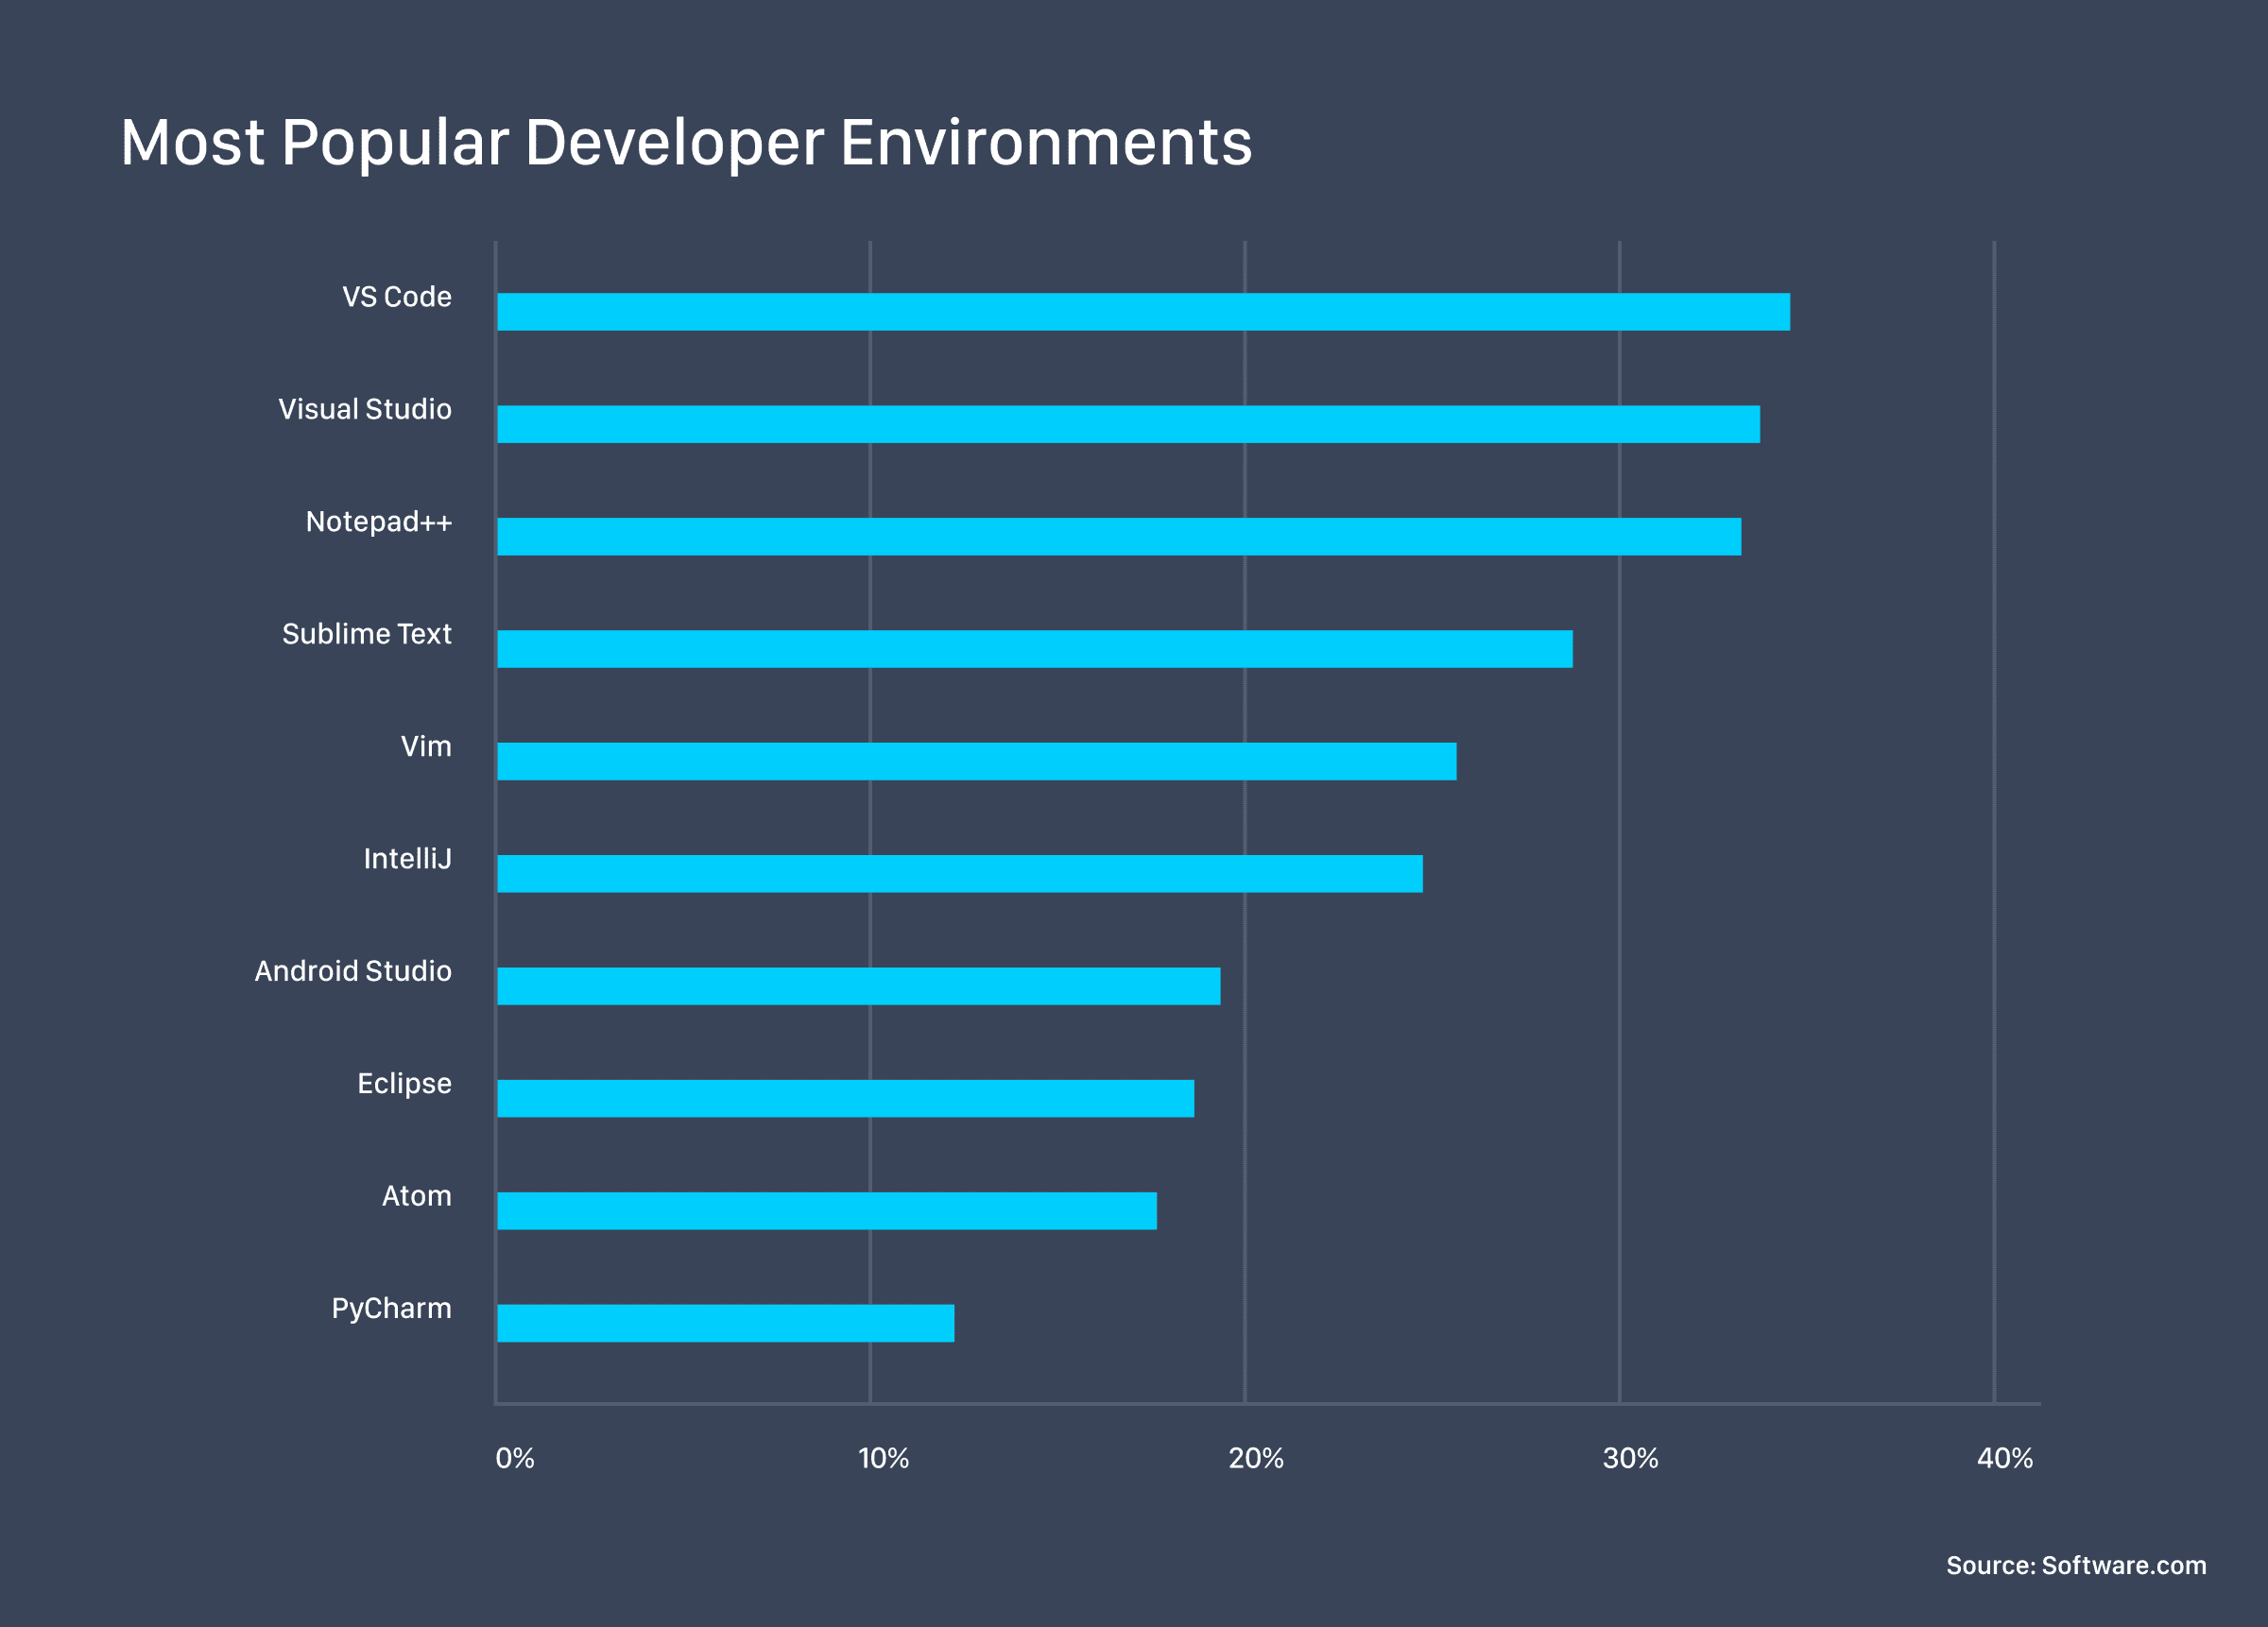
\includegraphics[width=0.6\linewidth]{fig/most-popular-dev-environments.png}
\end{figure}
\textbf{``Biggest ecosystem means more developers adding to value over time!''}
% https://www.software.com/src/ranking-the-top-5-code-editors-2019
\end{frame}

\begin{frame}{VS Code}
\begin{itemize}
	\item Official site: \url{https://code.visualstudio.com/}
	\item Keyboard shortcut: \url{https://code.visualstudio.com/shortcuts/keyboard-shortcuts-windows.pdf}
	\item New features in Chinese: \url{https://zhuanlan.zhihu.com/vs-code}
\end{itemize}
\end{frame}

\begin{frame}{Some features need to know}
\begin{itemize}
	\item Just open a folder w/o configuration
	\item Interface overview
	\item Interactive editor playground
	\item \href{https://code.visualstudio.com/docs/getstarted/tips-and-tricks\#vscode}{Tips and tricks}
\end{itemize}
\end{frame}

\begin{frame}{Regular Expression (regex)}
What is it?
\begin{flushleft}
A sequence of characters that define a search pattern used to find/replace sth. in strings.
\end{flushleft}
\begin{itemize}
	\item Tutorial: \url{https://github.com/ziishaned/learn-regex}
	\item Online test: \url{https://regex101.com}
\end{itemize}
\end{frame}

\begin{frame}{VS Code $\times$ Regex}
\begin{figure}
\centering

\includegraphics[width=\linewidth]{fig/vscode_regex.png}
\end{figure}
\end{frame}

\section{Environment Setting}
\begin{frame}
\sectionpage
\end{frame}

\begin{frame}{Use Unix-Like Environment!!!}
Why Linux?
\begin{itemize}
	\item Broken development tool chains on Windows
	\item Most of the packages are developed on Linux w/ little support to Windows
	\item All the severs use Linux environments
	\item * Exam/Competition system
\end{itemize}
\pause
Thus,
\begin{center}
\textcolor{red}{Get familiar with Linux!}
\end{center}
\end{frame}

\begin{frame}{Several Approaches}
\begin{itemize}[<+->]
	\item Buy an Apple computer with macOS!
	\begin{itemize}
		\item Expensive
	\end{itemize}
	\item Switch to a Linux system
	\begin{itemize}
		\item Time-consuming with backups to be made
	\end{itemize}
	\item Set up a dual system
	\begin{itemize}
		\item Unstable
	\end{itemize}
	\item Use a terminal emulator
	\begin{itemize}
		\item \href{http://www.msys2.org/}{MSYS2}, \href{https://www.cygwin.com/}{Cygwin}
		\item Not fully functional
	\end{itemize}
\end{itemize}
\end{frame}

\begin{frame}{Several Approaches (Cont.)}
\begin{itemize}[<+->]
	\item Install a virtual machine and use graphical user interface (GUI)
	\begin{itemize}
		\item \href{https://www.virtualbox.org/}{VirtualBox}, \href{https://www.vmware.com/}{VMWare}
		\item Very slow and memory-consuming
		\item \cmark, full system support with GUI \& portable
	\end{itemize}
	\item Use SSH to login in a remote server
	\begin{itemize}
		\item AWS, Azure, Google Cloud, Aliyun, Tencent Cloud
		\item \cmark, we will provide accounts of Lab servers later
	\end{itemize}
	\item Windows Subsystem for Linux (WSL)
	\begin{itemize}
		\item \cmark\cmark, easy to configure \& act like a real Linux!
	\end{itemize}
\end{itemize}
\end{frame}

\begin{frame}{No GUI, Use Terminal!}
Be familiar with terminal \& get rid of IDE!
\begin{itemize}
	\item Many packages have no GUI!
	\item Most of industrial server have no GUI
	\item GUI is very slow
	\item When you write huge projects, you have to configure all the settings \& dependency in Makefile and bash, which also has no GUI support.
\end{itemize}
\end{frame}

\begin{frame}{A Tradeoff $\ldots$}
Code on Windows w/ GUI, run on Linux w/o GUI
\begin{center}
\textbf{Windows Subsystem for Linux (WSL)}
\end{center}
\end{frame}

\begin{frame}{Windows Subsystem for Linux (WSL)}
Why WSL?
\begin{itemize}
	\item Very light-weight with most of Linux featues
	\item Efficient to have Windows \& Linux running together
	\item WSL 2 will be released in 2020 ($>$ Win 10 Build 18917)
\end{itemize}
Known issues: no support to perf \& GPU
\end{frame}

\begin{frame}{Begin with WSL}
Tutorial: \url{https://docs.microsoft.com/en-us/windows/wsl/install-win10}
\begin{itemize}
	\item Ubuntu LTS 18.04: Most commonly used (recommended!)
	\item Debian, CentOS: Enterprise
\end{itemize}
\end{frame}

\begin{frame}[fragile]{Ubuntu LTS 18.04}
\begin{figure}
\centering
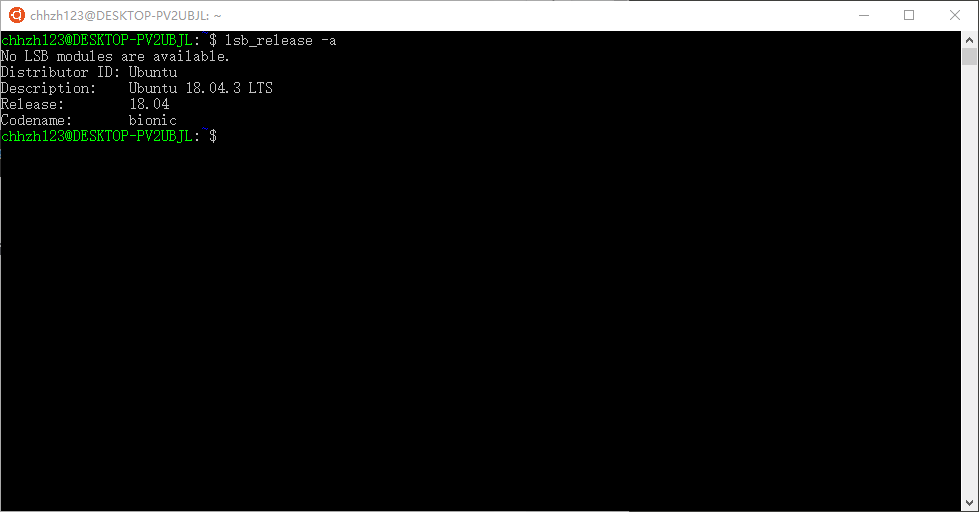
\includegraphics[width=0.8\linewidth]{fig/ubuntu_ver.png}
\end{figure}
Some difference between Unix \& Windows:
\begin{itemize}
	\item Line ending: \verb'\n' in Linux, \verb'\n\r' in Windows
	\item File path: \verb'/' in Linux, \verb'\\' in Windows
	\item WSL file system: \verb'/mnt/c'
\end{itemize}
\end{frame}

\begin{frame}[fragile]{Linux Command Lines (bash)}
Chinese tutorial: \url{https://linux.cn/article-6160-1.html}
\begin{itemize}
	\item \verb'cd' (w/ TAB usage)
	\item \verb'ls'
	\item \verb'mkdir'
	\item \verb'rm', \verb'cp', \verb'mv'
	\item \verb'apt-get'
	\item \verb'wget'
	\item \verb'vim'
\end{itemize}
Please get familar \& google for help.
\end{frame}

\begin{frame}{VS Code $\times$ WSL}
Install ``Remote - WSL'' in VS Code Extension
\begin{itemize}
	\item Workplace \& file path will change
	\item Full WSL support
\end{itemize}
\begin{figure}
\centering
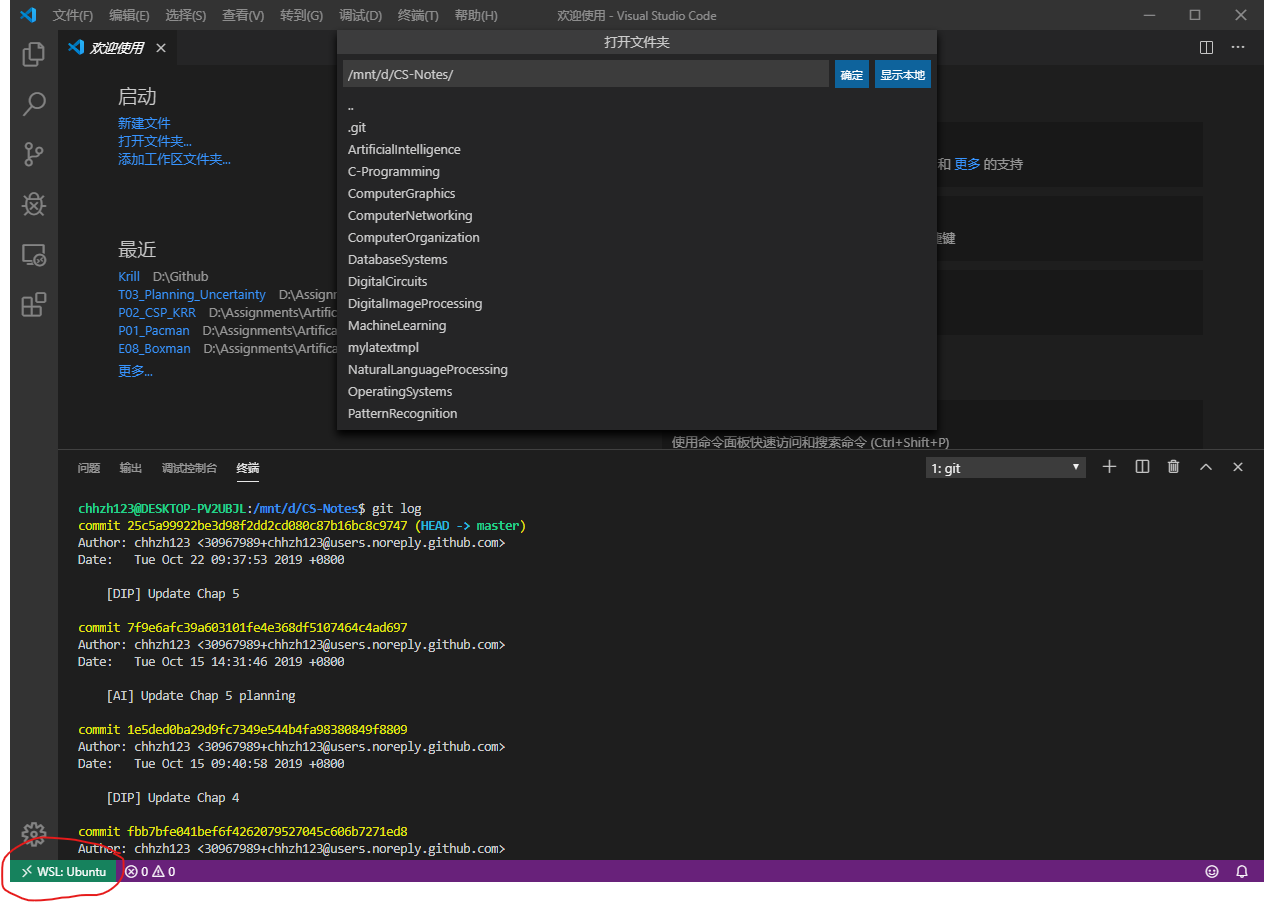
\includegraphics[width=0.6\linewidth]{fig/vscode_wsl.png}
\end{figure}
\end{frame}

\section{Code Management}
\begin{frame}
\sectionpage
\end{frame}

\begin{frame}{Git \& Github}
\begin{figure}
\centering
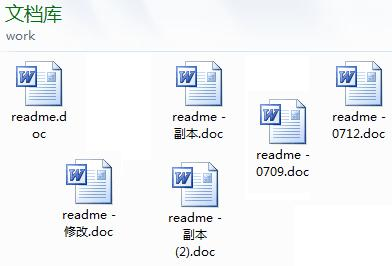
\includegraphics[width=0.5\linewidth]{fig/word-copy.jpg}
\caption*{Version control (pic via Xuefeng Liao)}
\end{figure}
\pause
\begin{center}
\Large \textbf{NO!!!}
\end{center}
\end{frame}

\begin{frame}{Git \& Github}
Then we have Git!
\begin{center}
\textbf{Git is a distributed version control system}
\end{center}
Some history:
\begin{itemize}[<+->]
	\item Linus created open-source Linux in 1991
	\item Before 2002, Linus merged codes from all over the world
	\item 2002-2005, used BitKeeper
	\item In 2005, Linus coded git in C in one month!
	\item In 2008, Github was created and became the most popular code management platform
\end{itemize}
\end{frame}

\begin{frame}[fragile]{Basic concepts of Git}
\textbf{Git is originally provided in Linux!}\\
Tutorial: \url{https://www.liaoxuefeng.com/wiki/896043488029600}
\begin{itemize}
\item Your repo
\begin{figure}
\centering
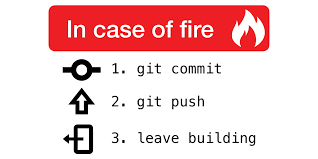
\includegraphics[width=0.6\linewidth]{fig/fire-git.png}
\end{figure}
\item Others' repo: \verb'git clone', \verb'git pull'
\end{itemize}
\end{frame}

\begin{frame}{Basic concepts of Git}
\only<1>{
\begin{figure}
\centering
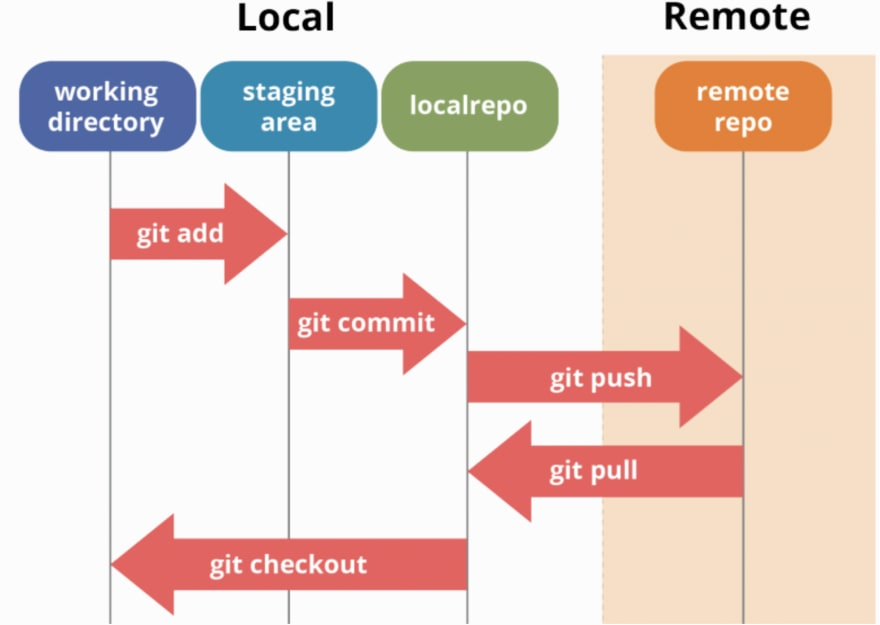
\includegraphics[width=0.7\linewidth]{fig/git_theory.jpg}
\end{figure}
}
\only<2>{
\begin{figure}
\centering
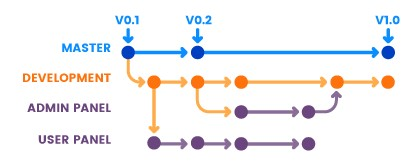
\includegraphics[width=0.8\linewidth]{fig/git-branches.jpg}
\end{figure}
\vspace{60pt}
\scriptsize * Pic via \url{https://rubygarage.org/blog/most-basic-git-commands-with-examples}
}
\end{frame}

\begin{frame}[fragile]{Basic concepts of Git}
\begin{itemize}
	\item \verb'.gitignore': ignore some files in your repository
	\begin{itemize}
		\item Generated/Intermediate files: \verb'.exe'
		\item Sensitive infomation
	\end{itemize}
	\item Submodule
\end{itemize}
\end{frame}

\begin{frame}[fragile]{Commit message}
A template: \url{https://blog.coding.net/blog/commit_message_change_log}
\begin{itemize}
	\item Be specific about what you have done in this commit
	\item DONT: \verb'1st commit', \verb'Commit', \verb'Message'
	\item DO: \verb'[DOC] fix typo in README.md'
\end{itemize}
\end{frame}

\begin{frame}{VS Code $\times$ Git}
Make sure your computer have Git installed
\end{frame}

\begin{frame}{Github}
The world's leading software development platform\\
(The biggest social networking platform (?))
\begin{figure}
\centering

\includegraphics[width=0.8\linewidth]{fig/microsoft-github-celebrate.jpg}
\end{figure}
\end{frame}

\begin{frame}{Start from Github}
\begin{figure}
\centering
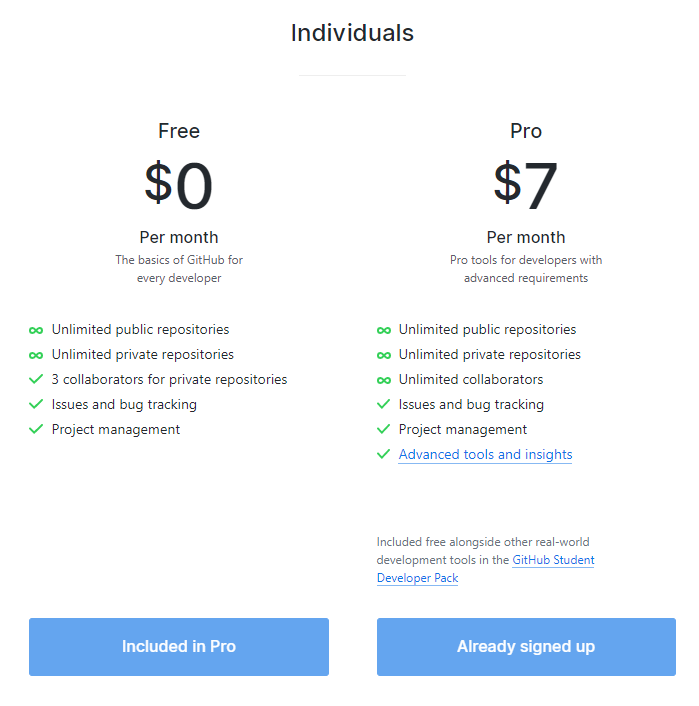
\includegraphics[width=0.8\linewidth]{fig/github_price.png}
\end{figure}
\end{frame}

\begin{frame}{Basic concepts of Github}
Some demo here $\ldots$
\begin{itemize}
	\item Repositories
	\item Projects:
	\begin{itemize}
		\item Watch, Star, Fork
		\item Issues, pull requests, merge requests
	\end{itemize}
\end{itemize}
\end{frame}

\begin{frame}{README Page}
Left to next course
% https://gist.github.com/PurpleBooth/109311bb0361f32d87a2
\end{frame}

\begin{frame}{Licenses}
Commonly used licenses: \url{https://choosealicense.com/licenses/}
% https://www.freecodecamp.org/news/how-open-source-licenses-work-and-how-to-add-them-to-your-projects-34310c3cf94/
\begin{itemize}
	\item When you use others' code, please view licenses
	\item The most restrictive licenses is GPL
	\item The most permissive licenses is MIT
	\item Other popular licenses are Apache License 2.0 and BSD
	\item Your daily-life project needs not add licenses
\end{itemize}
\end{frame}

\section{Code Specification}
\begin{frame}
\sectionpage
\end{frame}

\begin{frame}[fragile]{Style notes}
Key: \textbf{Style in one way!}
\begin{itemize}
	\item Variable naming convention
	\begin{itemize}
		\item Camel case: \verb'newString'
		\item Pascal case: \verb'NewString'
		\item Underline: \verb'new_string'
	\end{itemize}
	\item Empty space / newlines are needed
	\begin{itemize}
		\item \verb'for (i = 0; i < 10; ++i)'
		\item Newline bracket or not depends on yourself
		\item Use space \& empty lines to separate different code sections
	\end{itemize}
	\item Please be specific (or you will not pass vmatrix)
	\begin{itemize}
		\item DO: \verb'wordLen', \verb'drawImage()'
		\item DONT: \verb'a', \verb'aaaaa', \verb'method1'
	\end{itemize}
	\item \textbf{Add comments} unless what your code does is evident
	\item Please \textbf{use English} (utf-8) all the way!
\end{itemize}
\end{frame}

\begin{frame}{Google Style Guide}
Google Style Guide: \url{http://google.github.io/styleguide/}
\begin{itemize}
	\item Need not be rigorous, but please keep ONE format in one project
	\item Using formatting in VS Code is enough
\end{itemize}
\end{frame}

\section{Summary}
\begin{frame}
\sectionpage
\end{frame}

\begin{frame}{Summary of Week 1 - Basic Configuration}
\begin{itemize}
	\item Text Editors: VS Code/Vim, regular expression
	\item Environment: Linux (WSL), bash
	\item Code management: git, Github
	\item Code spec: Google Style Guide
\end{itemize}
\end{frame}

\begin{frame}[fragile]{Assignments}
Clone this seminar via
\begin{flushleft}
\scriptsize \verb'git clone --recursive https://github.com/chhzh123/ToolsSeminar-CS.git'
\end{flushleft}
\begin{enumerate}
	\item Be familiar with Text editors which you may use every day
	\item Have a Linux machine \& learn basic bash commands
	\item Register a Github account and take a look of Github
	\item Finish assignment on easy \textbf{string matching}
	\item Create a repository to store assignments of this seminar
	\item Upload your assignments to Github
\end{enumerate}
Details can be found in \verb'Materials-BasicConfiguration.pdf'.
\end{frame}

\end{document}